% Options for packages loaded elsewhere
\PassOptionsToPackage{unicode}{hyperref}
\PassOptionsToPackage{hyphens}{url}
%
\documentclass[
]{article}
\title{Creating a Treemap}
\author{Hanna}
\date{2022-12-02}

\usepackage{amsmath,amssymb}
\usepackage{lmodern}
\usepackage{iftex}
\ifPDFTeX
  \usepackage[T1]{fontenc}
  \usepackage[utf8]{inputenc}
  \usepackage{textcomp} % provide euro and other symbols
\else % if luatex or xetex
  \usepackage{unicode-math}
  \defaultfontfeatures{Scale=MatchLowercase}
  \defaultfontfeatures[\rmfamily]{Ligatures=TeX,Scale=1}
\fi
% Use upquote if available, for straight quotes in verbatim environments
\IfFileExists{upquote.sty}{\usepackage{upquote}}{}
\IfFileExists{microtype.sty}{% use microtype if available
  \usepackage[]{microtype}
  \UseMicrotypeSet[protrusion]{basicmath} % disable protrusion for tt fonts
}{}
\makeatletter
\@ifundefined{KOMAClassName}{% if non-KOMA class
  \IfFileExists{parskip.sty}{%
    \usepackage{parskip}
  }{% else
    \setlength{\parindent}{0pt}
    \setlength{\parskip}{6pt plus 2pt minus 1pt}}
}{% if KOMA class
  \KOMAoptions{parskip=half}}
\makeatother
\usepackage{xcolor}
\IfFileExists{xurl.sty}{\usepackage{xurl}}{} % add URL line breaks if available
\IfFileExists{bookmark.sty}{\usepackage{bookmark}}{\usepackage{hyperref}}
\hypersetup{
  pdftitle={Creating a Treemap},
  pdfauthor={Hanna},
  hidelinks,
  pdfcreator={LaTeX via pandoc}}
\urlstyle{same} % disable monospaced font for URLs
\usepackage[margin=1in]{geometry}
\usepackage{graphicx}
\makeatletter
\def\maxwidth{\ifdim\Gin@nat@width>\linewidth\linewidth\else\Gin@nat@width\fi}
\def\maxheight{\ifdim\Gin@nat@height>\textheight\textheight\else\Gin@nat@height\fi}
\makeatother
% Scale images if necessary, so that they will not overflow the page
% margins by default, and it is still possible to overwrite the defaults
% using explicit options in \includegraphics[width, height, ...]{}
\setkeys{Gin}{width=\maxwidth,height=\maxheight,keepaspectratio}
% Set default figure placement to htbp
\makeatletter
\def\fps@figure{htbp}
\makeatother
\setlength{\emergencystretch}{3em} % prevent overfull lines
\providecommand{\tightlist}{%
  \setlength{\itemsep}{0pt}\setlength{\parskip}{0pt}}
\setcounter{secnumdepth}{-\maxdimen} % remove section numbering
\ifLuaTeX
  \usepackage{selnolig}  % disable illegal ligatures
\fi

\begin{document}
\maketitle

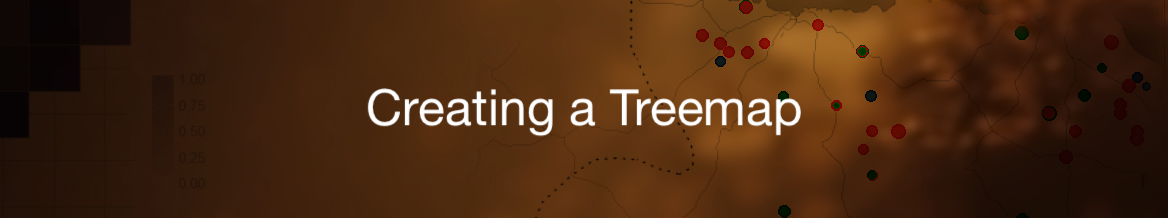
\includegraphics{tutorialhead.png}

\hypertarget{tutorial-aims}{%
\subsection{Tutorial Aims:}\label{tutorial-aims}}

\hypertarget{develop-a-good-understanding-of-treemaps-and-how-they-are-useful}{%
\paragraph{1.Develop a good understanding of Treemaps and how they are
useful}\label{develop-a-good-understanding-of-treemaps-and-how-they-are-useful}}

\hypertarget{understand-how-to-upload-data-into-your-r-studio}{%
\paragraph{2.Understand how to upload data into your R
Studio}\label{understand-how-to-upload-data-into-your-r-studio}}

\hypertarget{be-able-to-transform-data-into-a-treemap}{%
\paragraph{3.Be able to transform data into a
Treemap}\label{be-able-to-transform-data-into-a-treemap}}

\hypertarget{be-able-to-change-the-appearance-of-a-treemap}{%
\paragraph{4.Be able to change the appearance of a
Treemap}\label{be-able-to-change-the-appearance-of-a-treemap}}

\hypertarget{steps}{%
\subsection{Steps:}\label{steps}}

\hypertarget{loading-needed-packages}{%
\paragraph{\texorpdfstring{ 1. Loading needed packages
}{ 1. Loading needed packages }}\label{loading-needed-packages}}

\hypertarget{downloading-data}{%
\paragraph{\texorpdfstring{ 2. Downloading
data}{ 2. Downloading data}}\label{downloading-data}}

\hypertarget{creating-the-treemap}{%
\paragraph{\texorpdfstring{ 3. Creating the
Treemap}{ 3. Creating the Treemap}}\label{creating-the-treemap}}

\hypertarget{changing-your-treemaps-look}{%
\paragraph{\texorpdfstring{ 4. Changing your Treemaps
look}{ 4. Changing your Treemaps look}}\label{changing-your-treemaps-look}}

\hypertarget{making-your-treemap-more-interactive}{%
\paragraph{\texorpdfstring{ 5. Making your Treemap more
interactive}{ 5. Making your Treemap more interactive}}\label{making-your-treemap-more-interactive}}

\hypertarget{more-sources}{%
\paragraph{\texorpdfstring{ 6. More
sources}{ 6. More sources}}\label{more-sources}}

\hypertarget{what-is-a-treemap}{%
\subsection{What is a Treemap?}\label{what-is-a-treemap}}

In its most basic form, a Treemap is used to visualize proportions.
Similar to a pie chart, a Treemap allows the reader to see different
values as part of a whole, in this case a large rectangle instead of a
circle. Treemaps are also super useful to display lots of information in
a small amount of space. Using hierarchical Treemaps allow the plot to
interactive and show different kinds of information.

Treemaps can come in multiple forms ranging from very basic to very
complex. Today you will be learning the most basic kind of Treemap and
how to make it interactive.

\hypertarget{loading-needed-packages-1}{%
\subsection{1. Loading needed
packages}\label{loading-needed-packages-1}}

For this tutorial you will need 5 different packages. Copy the code
below into your RStudio and run it to install and load the needed
package.

\texttt{install.packages("tidyverse")}

\texttt{install.packages("treemap")}

\texttt{install.packages("dplyr")}

\texttt{install.packages("readr")}

\texttt{install.packages("d3treeR")}

\texttt{devtools::install\_github("timelyportfolio/d3treeR")\ \#\ use\ this\ code\ if\ d3treeR\ does\ not\ install\ on\ the\ first\ try\ (remove\ the\ \#\ to\ run\ this\ code)}

Once you have installed these packages it is time to load them up. Use
the code below to do that.

\texttt{library(tidyverse)}

\texttt{library(treemap)}

\texttt{library(dplyr)}

\texttt{library(readr)}

\texttt{library(d3treeR)}

\hypertarget{downloading-data-1}{%
\subsection{2. Downloading data}\label{downloading-data-1}}

To get the needed data,
\href{https://github.com/EdDataScienceEES/tutorial-Hannalh14}{please
visit this repository}. Once you have copied the repo, please set your
working directory to where you saved it on your device. Use the
following code to set your working directory.

\texttt{setwd("You\_file\_path")}

The next step in this process is to load the data from the repo and view
it in your RStudio. Use the code below to do that.

\texttt{popdata\ \textless{}-\ read.csv("us\_pop\_by\_state.csv")}

\texttt{view(popdata)}

An important thing to keep in mind if you decide to make a Treemap with
your own data is to make sure your data is compatable. To make a Treemap
you need to have hierarchical data.Sort of like a nesting doll or an
onion, data with various layers wrok well when creating Treemaps. In
this tutorial you with be working with very very simple data that have
very few layers.W will be using the US states and their populations
recorded from the 2020 census. Something else to keep in mind if you are
to use this method with your own data is to make sure the data doesn't
have a total sum of your values. For example, the entire population of
the US. This total can throw off the proportions of your Treemap so it
is best to get rid of it.

Below you can see an example of a Treemap if we did not get rid of the
whole population of the US.

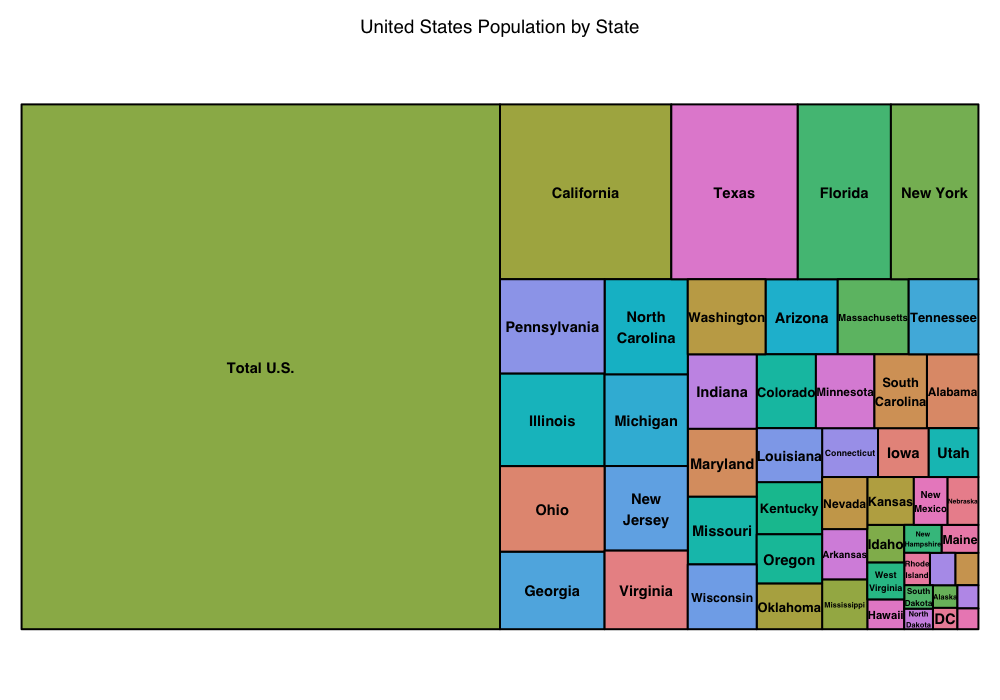
\includegraphics{wholepopplot.png} To avoid this, we need to get rid of
this total in our data. That can be done with the code below. Note: this
code does gets rid of the territory of Washington D.C. This data collect
D.C. as its own district so we will be keeping it to make the data
consistent.

\texttt{statepop\ \textless{}-\ popdata\ \%\textgreater{}\%\ slice(-c(52))}
\texttt{view(statepop)}

As you can see when you view the data, the last row has been removed.

This can also be relevant with observational data, you do not want a row
that contains a sum of all of your observations.

\hypertarget{creating-the-treemap-1}{%
\subsection{3. Creating the Treemap}\label{creating-the-treemap-1}}

Now that our data is all sorted, it is time to create the Treemap.
First, it is good to have an understanding of the code you will be
running. We will be using the Treemap package you downloaded at the
beginning of this tutorial. As you can see in the code you are going to
run below, you must call both the Treemap package and the data that we
sliced above. Some other important aspects to understand are what pieces
of the data youa re using to create this plot.''Index'' is referring to
the characters we are comparing, in this case it will be the US states.
``vSize'' is the numerical values we are comparing, in this instance it
is the population from the 2020 census. Next is ``type'' that is just
determining the color scheme used in the Treemap. Lastly, is title which
is pretty self explanitory.

The code below will result in your first Treemap! Try it out!

poptm \textless- treemap(statepop,

\begin{verbatim}
              index = c("state"),
              
              vSize = "X2020_census",
              
              type= "index",
              
              title = "United States Population by State")
              
\end{verbatim}

You should have gotten something that looks like this.

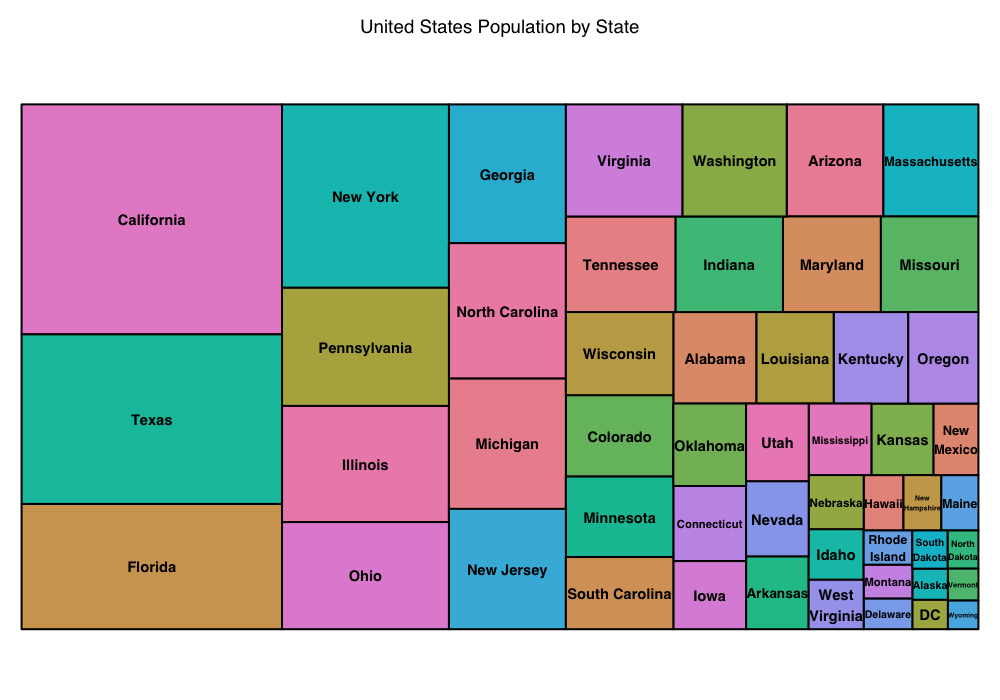
\includegraphics{plotfullname.png} With all of those names of those
states the Treemap has gotten a little crowded. something you want to
ensure when making a Treemap is that it is legible, this means both the
identifiers (the states names), and the visual proportions are easy to
read. In the dataset you have retrieved there is another way to identify
these states that is a better visualization of the data. Try the code
below to see this new map.

abvtm \textless- treemap(statepop,

\begin{verbatim}
             index = c("state_code"),
             
             vSize = "X2020_census",
             
             type = "index",
             
             title = "United States Population by State")
\end{verbatim}

` You should see something like this.

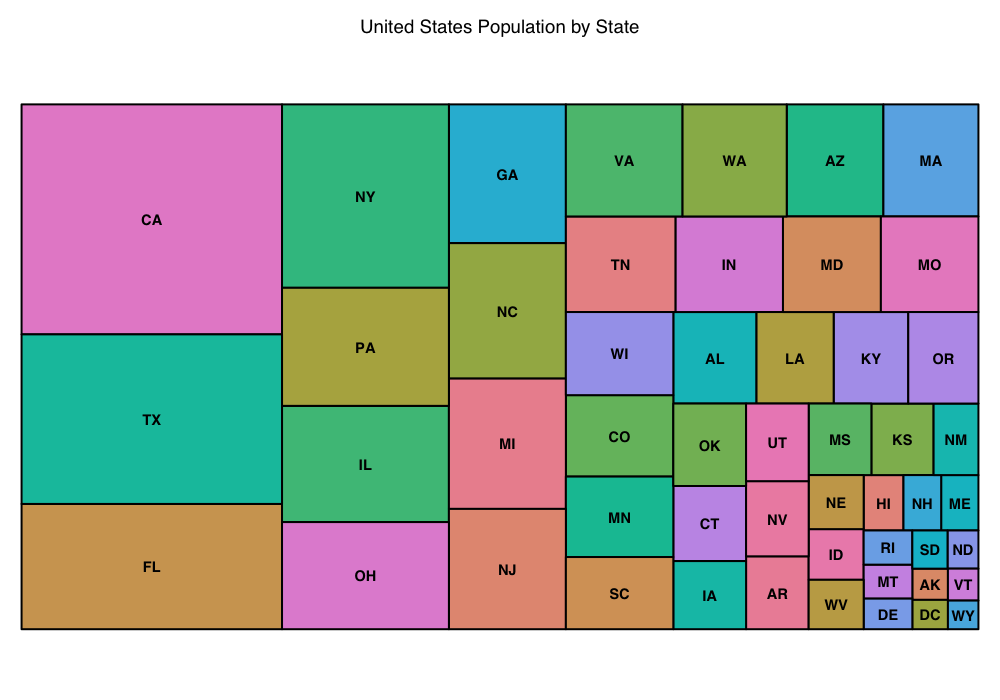
\includegraphics{abrvtreemap.png}

\hypertarget{changing-your-treemaps-look-1}{%
\subsection{4. Changing your Treemaps
look}\label{changing-your-treemaps-look-1}}

Like all plots, the most fun part about creating them is being able to
make them look really nice and fun! Below is the code for a similar map
to before with some different aspects changed. There are many different
color palettes to choose from, check out
\href{https://www.datanovia.com/en/blog/the-a-z-of-rcolorbrewer-palette/\#:~:text=RColorBrewer\%20is\%20an\%20R\%20package,Install\%20and\%20load\%20RcolorBrewer\%20package}{this
link} for some palette inspiration, or try your hand at making your own
color palette!

The code below changes the color palette and also secures the font and
border colors for this Treemap. Give it a go!

tmcolorp \textless- treemap(statepop,

\begin{verbatim}
               index = c("state_code"),
               
               vSize = "X2020_census",
               
               type = "index",
               
               title = "United States Population by State",
               
               palette = "Spectral",
               
               border.col = "black",
               
               fontcolor.labels = "black")
\end{verbatim}

\hypertarget{making-your-treemap-interactive}{%
\subsection{5. Making your Treemap
interactive}\label{making-your-treemap-interactive}}

Treemaps have the potential to be very complex and elaborate. Today we
made a very basic Treemap, but that doesn't mean we can't spruce it up
just a little but more and make it more informative. The code below uses
a package called ``d3treeR'', this package allows you to make
interactive Treemaps. This allows your Treemap to have more information
and still look neat on the outside. To see more of these interactive
Treemaps, please see the reading below.

Give this code a try!

United\_States\_Population\_by\_State \textless- tmcolorp \#This renames
the previous plot so it will show up as the heading.

d3tree2(United\_States\_Population\_by\_State)

As you can see the actual populations of each state show up when you put
your curser over the states section. This interactive feature would work
even better with dense hierarchical data. If you wish to explore this
feature more check out these two sources! Using
\href{https://plotly.com/r/treemaps/}{Plotly} and using
\href{https://d3-graph-gallery.com/treemap.html}{d3tree}

\hypertarget{learn-more-with-these-sources}{%
\subsection{Learn more with these
sources!}\label{learn-more-with-these-sources}}

\href{https://r-graph-gallery.com/236-custom-your-treemap}{More basics
of Treemaps}

\href{https://www.r-bloggers.com/2018/09/simple-steps-to-create-treemap-in-r/}{Treemap
reading}

\href{https://www.data-to-viz.com/caveat/pie.html}{Why Treemaps are
better than pie charts}

\end{document}
